\section*{Introduction}
%------------------------------------------------------------------------------
%------------------------------------------------------------------------------

% \subsection*{Estuaries and Phytoplankton}

\texttt{Add a short paragraph as an outlook of the paper? I was told thats what the cool kids do but I feel like thats already in the abstract.}


Estuaries are important both for the climate system as well as for anthropogenic use.
From a climate perspective they are highly productive relative to their surface area 
which results in large amounts of direct carbon cycling 
along with their important role as a source of nutrients and hatching grounds for marine ecosystem. (cite)
They are also strongly anthropogenically influenced through e.g. harbors, diking, dredging, fishing and pollution which can be seen as a stressor on the ecosystem but it also adds an anthropogenic dependency on the ecosystem. (cite)

Estuaries are also complex and strongly dynamic systems such that it is still difficult to predict ecosystem dynamics or the effects of anthropogenic changes. (cite)
This complexity arises in part from the bathymetrie and the resulting hydrodynamics at the fresh-salt water interface. (cite)

As for most ecosystem - their dynamics are strongly controlled by the primary producers.
Phytoplankton, the 	predominant aquatic primary producer is mostly drifting passively through the water.
Hence, its trajectory is strongly controlled by the currents and tides.
With the estuary having a net outwards flow we expect phytoplankton to be moving
 downstream over time and ultimately to be washed out into marine high salinity waters.
Therefore, we are wondering how phytoplankton manages to survive as a population in such an environment.
If we assume that the population is not exclusively maintained by upstream plankton that is washed into the estuary
 then there must be some sort of retention mechanism that enables a phytoplankton population to remain in the low-salinity area of the estuary.
While we suspect that such a mechanism is crucial for survival it is currently not well understood 
due to the difficulty in either measuring or modeling such processes.



% \subsection*{Current state of knowledge}


We categorize the already performed studies on the subject of phytoplankton retention in three groups: observations, theoretical- and applied-modelling.

Observational studies have found three major mechanism for retention - sinking, diel migration, and stickiness. (cite)
Diel migration - moving up and down with the sun -  has been found to be favorable for retention by allowing organisms to stay close to bottoms slow moving waters.
However, so far this has only shown for larger motile estuarine organisms i.e. zooplankton species [cite].
Benthic phytoplankton especially has been observed to be strongly negatively buoyant, hence sinking to the ground and remaining there for a long time (cite).
Recent studies also found sticky compounds in phytoplankton aggregates that are suspected to let them stick to themselves and their surroundings aiding retention. (cite)



Next we want to highlight several modelling study that examined whether certain retention mechanism could work in theory.
Two theoretical modelling studies studying the mechanisms of "loss compensation" and "reseeding".
\texttt{I don't like the term theoretical modelling study. Maybe "conceptual", "abstract" or "simple"?}
(cite) theorized a set up in which a population is able to maintain itself if the losses due to outwashing can be compensated by growth.
In a setup where a lagoon like ecosystem was modelled they were able to quantify reproduction thresholds that are needed to maintain the population.
However, this setup also implies that the growing part of the population is somehow retaining their position.
If the regrowing population is also continuously drifting downstream they will also ultimately die out.
(cite) studied the concept of "reseeding".
Here a system is theorized in which a population is able to repopulate an previously 
lost or uncolonized area upstream due to local upstream currents e.g. through tides or dispersion.
While they showed that upstream reseeding is conceptually possible they did so in a specifically contrived system resembling groyne fields .
Whether this is an actual realized phenomenon depends on the topology and hydrodynamic of the estuary.
Nevertheless, it has been shown that both "outgrowing the losses" and "reseeding" are possible retention mechanism under certain conditions.

In (cite) they use a particle tracking model also known as Lagragian model to study Zooplankton movement in the San Francisco Bay.
They were able to show  that sinking and diel migration slows the outwashing process and might be beneficial retention tactic.
However, they did so by ignoring key processes like reproduction, mortality and any stranding or sedimentation processes in an low resolution structured grid model.

We are examining the Elbe estuary as a case study.
Like most alluvial estuaries it is relatively flat.
Similar to other European estuaries it experienced a strong anthropogenic pressure over the last centauries.
Most notably diking to restrain it to a narrow channel and dreading to improve access to the Hamburg harbor.
Unlike other major european harbors, the Hamburg harbor is located far inwards roughly 100km away from the coast.
This causes the river to experience a sudden jump in bathymetry from 5m at border of the city to almost 20m in the harbor (see fig. \ref{fig:bathymetry}). 
This bathymetric jump is suspected to be the cause of a collapse of the phytoplankton biomass causing an increase in oxygen depletion and high ammonium reminaralization after the bathymetric jump. (cite)
While major aspects of the along-channel biochemical dynamics have been studied little is known regarding their vertical and shore-to-shore dynamics.

\begin{figure}
    
\includegraphics[width=\columnwidth]{harbor.png}
    \caption{Bathymetry of the Elbe model around Hamburg. Note the bathymetric jumps from ~5m on the right, upstream side to a short 10m step in the upper harbor area to the ~20m in the lower harbor area all the way to the north sea. Also note that there exists no channel that does not pass through the 10km long exclusively 20m deep area. }
    \label{fig:bathymetry}
\end{figure}

To summarize - several concepts for potential retention mechanisms have been found
 and shown to work in certain conditions.
However, all approaches used major simplification which didn't allow them to study the full picture.
We developed a new and more realistic approach to study retention using a particle tracking model.
This model combines the features outlined above, namely: reproduction, mortality, vertical migration, stranding, sedimentation, and reseeding.
We examine if such a system can reproduce phytoplankton retention in the Elbe estuary with these mechanisms and if so under which conditions.




\section*{Methods}
%------------------------------------------------------------------------------
%------------------------------------------------------------------------------

\subsection*{Model description}

\subsubsection*{Particle tracking}

In our study we take a particle tracking approach with a lagrangian model called Oceantracker (cite).
Particle tracking offers several advantages for our question:
While particle tracking on unstructured grids has been relatively computationally expensive until recently (cite).
it allows us to reuse already validated hydrodynamic models.
Reusing already computed hydrodynamical models to study tracer like objects with an Lagrangian model  is overall much faster than recalculating the advection-diffusion-equation in an Eularian model.

Additionally, because we are simulating individually particles we are able to observe their tracks.
This makes it much easier and intuitive to interpret the results and allows us to include individual based properties and processes.

\subsubsection*{Hydrological model}
We use the hydrodynamics data of the most recent SCHISM model (cite Johannes Pein).
It is an three dimensional unstructured  grid model representing the full Elbe estuary from the weir at Geesthacht close to Helgoland including side-channels and the harbor (see fig. \ref{fig:model_domain}). 
% (Look for more details in pein paper that might be interesting)
The model provides a node-based mesh field containing a range of information.
Most important for our purpose is the water velocity.
But also salinity, water level, dispersion and many other more technical properties are used (See appendix \texttt{not yet added})
The year represented in that dataset is 2012 with 1h temporal- and dynamically varying spacial resolution with a median distance between nodes of $\sim60m$.

\begin{figure}
    \includegraphics[width=\columnwidth]{dfg_foto_wettbewerbg_laurin_legendless_steidle_small.png}
    \caption{Map of the full model domain with Geesthacht being the upstream boarder on the right and the Northsea being the downstream edge on the top left. The gray outline indicates the edge of the model domain. Blue and green dots show an example snapshot of a phytoplankton distribution in the model. Blue being floating, green being stranded particles.}
    \label{fig:model_domain}
\end{figure}

\subsubsection*{Particle based processes}

On top of the "blank" particle we add a set of biological features to achieve a more realistic behavior.
The most important one is their ability to reproduce by creating copies of themselves.
This is represented as a constant chance of duplicating a particle.
We also remove them under certain biologically unfavorable conditions. Specifically when they are stranded on the shore, starved for light or float in high salinity waters for too long.
More precisely, they are removed if either of the following criteria is met: 
When they reach high salinity waters implemented as a mortality chance $1\%$ every minute.
of  in fixed intervals above $10$PSU.
When they are stranded outside of the water and lie dry for more then $7$ consecutive days.
When they are starved for light which is represented as a budget of $14$ days 
where energy is lost in a fixed rate in low-light and gained in high light areas.

A set of vertical movement features is added to model migration behavior. 
This is implemented in two modes. 
One being a constant vertical velocity i.e. sinking and rising
The second being diel-migration where they move up and down depending on the phase of the sun.
A large area of the estuary is very shallow with average water depths of below one meter. 
We include a simple sedimentation and resuspension model to represent stranding by the tide and also sedimentation model for the water column where resupension is depending on a critical sheer velocity (see appendix).

Particles are stranded and temporarily stuck in place when they cross a model boundary or when their current cell falls dry. 
Particle are resuspended from the bottom based on a critical sheer velocity model.
If they are stranded they resuspend as soon as there location is flooded again.

The model also implements dynamic dispersion that is crucial to represent tidal-pumping processes and to allow for more realistic trajectories.

\subsection*{Experimental configurations}

The first experiment of this study examines retention success under different scenarios.
The general idea is to release a population of plankton at the upstream end of the estuary represented by the weir in Geesthacht
and examine how the population distrubutes itself over the estuary and whether it is able to maintain its population size.
% With this approach we study the effect of two retention mechanism in a sensitivity analysis. These being reproduction and migration.

The initial particle batch that is representing our phytoplankton population is released at the beginning of the year in a volume at the weir in Geesthacht which marks the beginning of the Estuary.
We evaluate their retention success by counting the amount of plankton in different regions in the estuary over time.
If the population is growing at the end of the year we consider them "successfully retained".
Population changes are measured at the end of the year relative to the population size after after an initial spin up time of three months where most of the initial batch has been washed out and the population is typically at its minimum.

For each particle we log their distance traveled, age, water depth, and status - whether they are drifting, stranded on the shore or bottom.
This allows us to compare the successful (died older then three months) and unsuccessful (died younger then three months ) plankton.
The logged observables are measured every 12 hours starting at midnight.

\medskip

We use this set-up in a range of scenarios.
We call the first and simplest scenario "dust". 
Here we don not allow for any reproduction and give all particles a neutral buoyancy.
Hence they are drifting like dust similar to a passive tracer
This is our reference for any retention strategy. 
For a retention strategy to be considered beneficial it must perform better than these passive tracers.

In the second scenario referred to as "migration" reproduction is re-enabled.
In this scenario we study the effect of different growth rates and buoyancies i.e. vertical velocities on the phytoplankton population in a sensitivity analysis.

The third scenario has been added for illustration purposes.
Here, we use the same set-up as in the second scenario with the only exception of disabling reproduction for particles stranded on the shores of the estuaries.

% \subsubsection*{upstream migration}

% In the second and minor experiment we test the hypothesis of "reseeding" - whether organisms can recolonize previously lost upstream habitats.
% \texttt{This is currently not included anymore. Seemed to uninteresting and far off track. What do you think?}


\section*{Results}
%------------------------------------------------------------------------------
%------------------------------------------------------------------------------

\subsection*{Retentions experiments}

\subsubsection*{Scenario: dust, mono- and diel migration}

\begin{figure}
    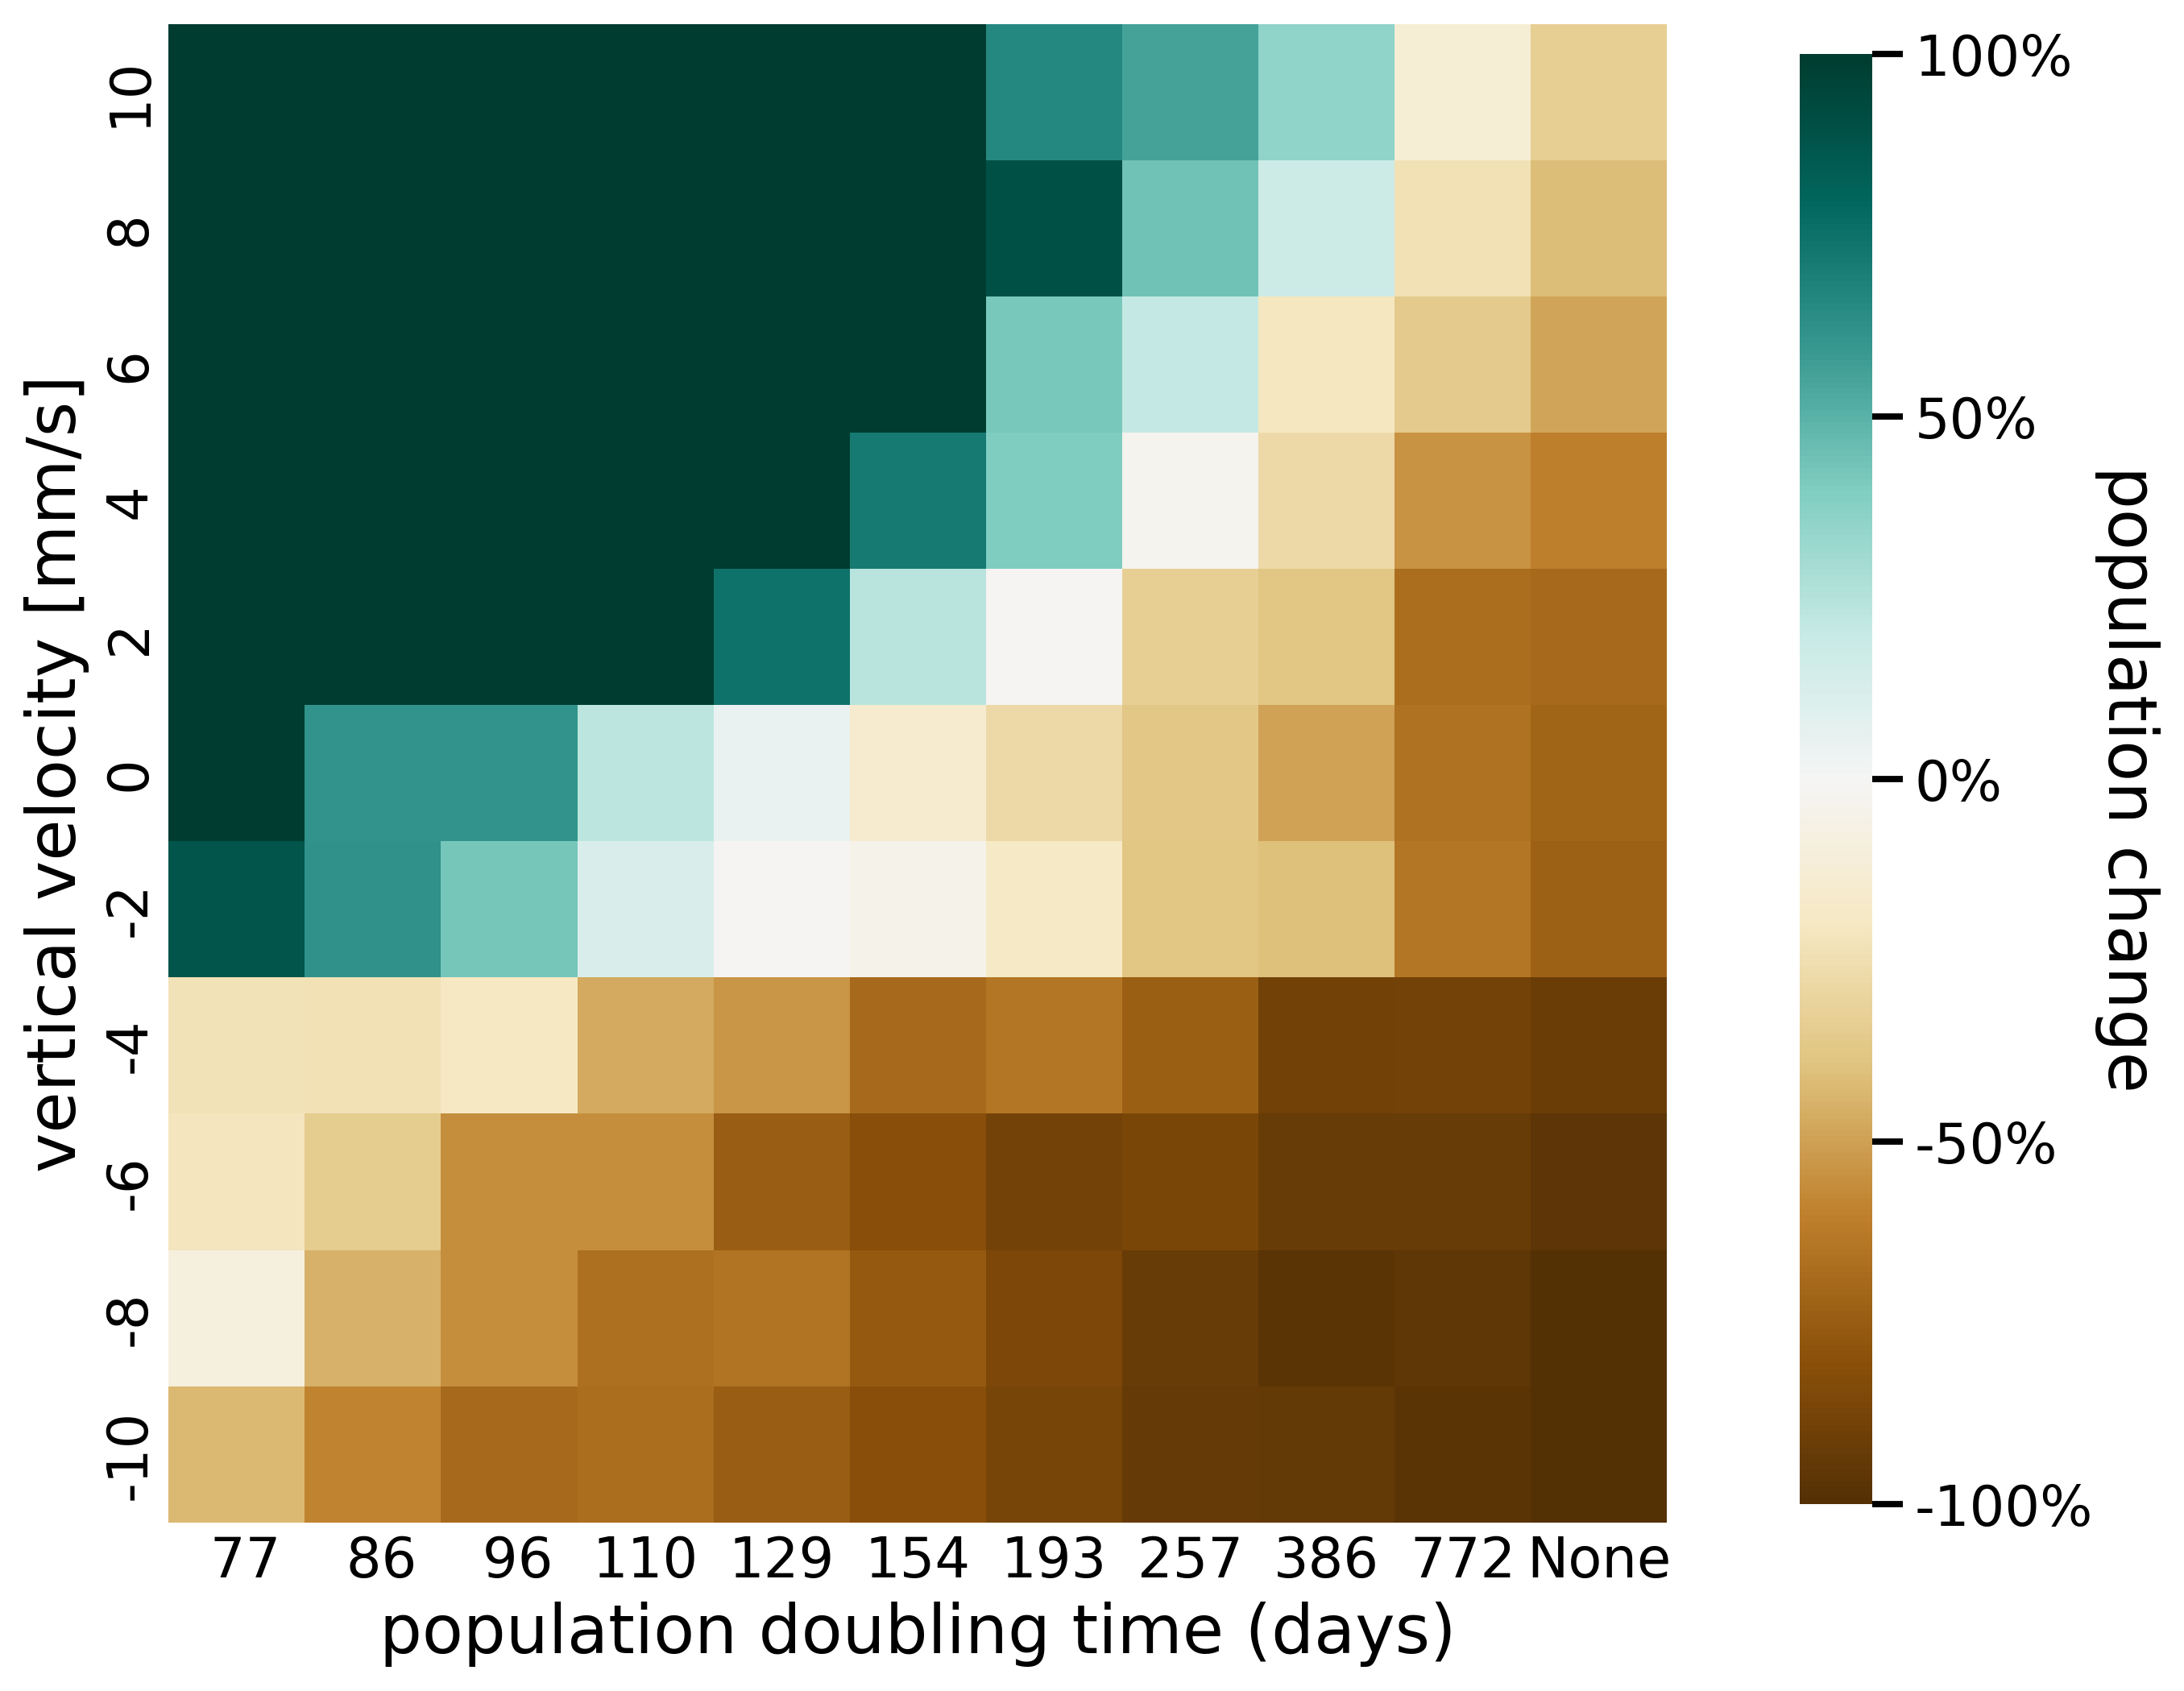
\includegraphics[width=\columnwidth]{retention_success_sa_mono.png}
    \caption[]{Relative population changes for the monotonic migration scenarios. Positive vertical velocities indicate an upwards drift direction. Positive population changes indicate a retention success (shown in green) while negative population changes predict a long term loss of the population (shown in brown).}
    \label{fig:monotonic_retention_success}
\end{figure}
\begin{figure}
    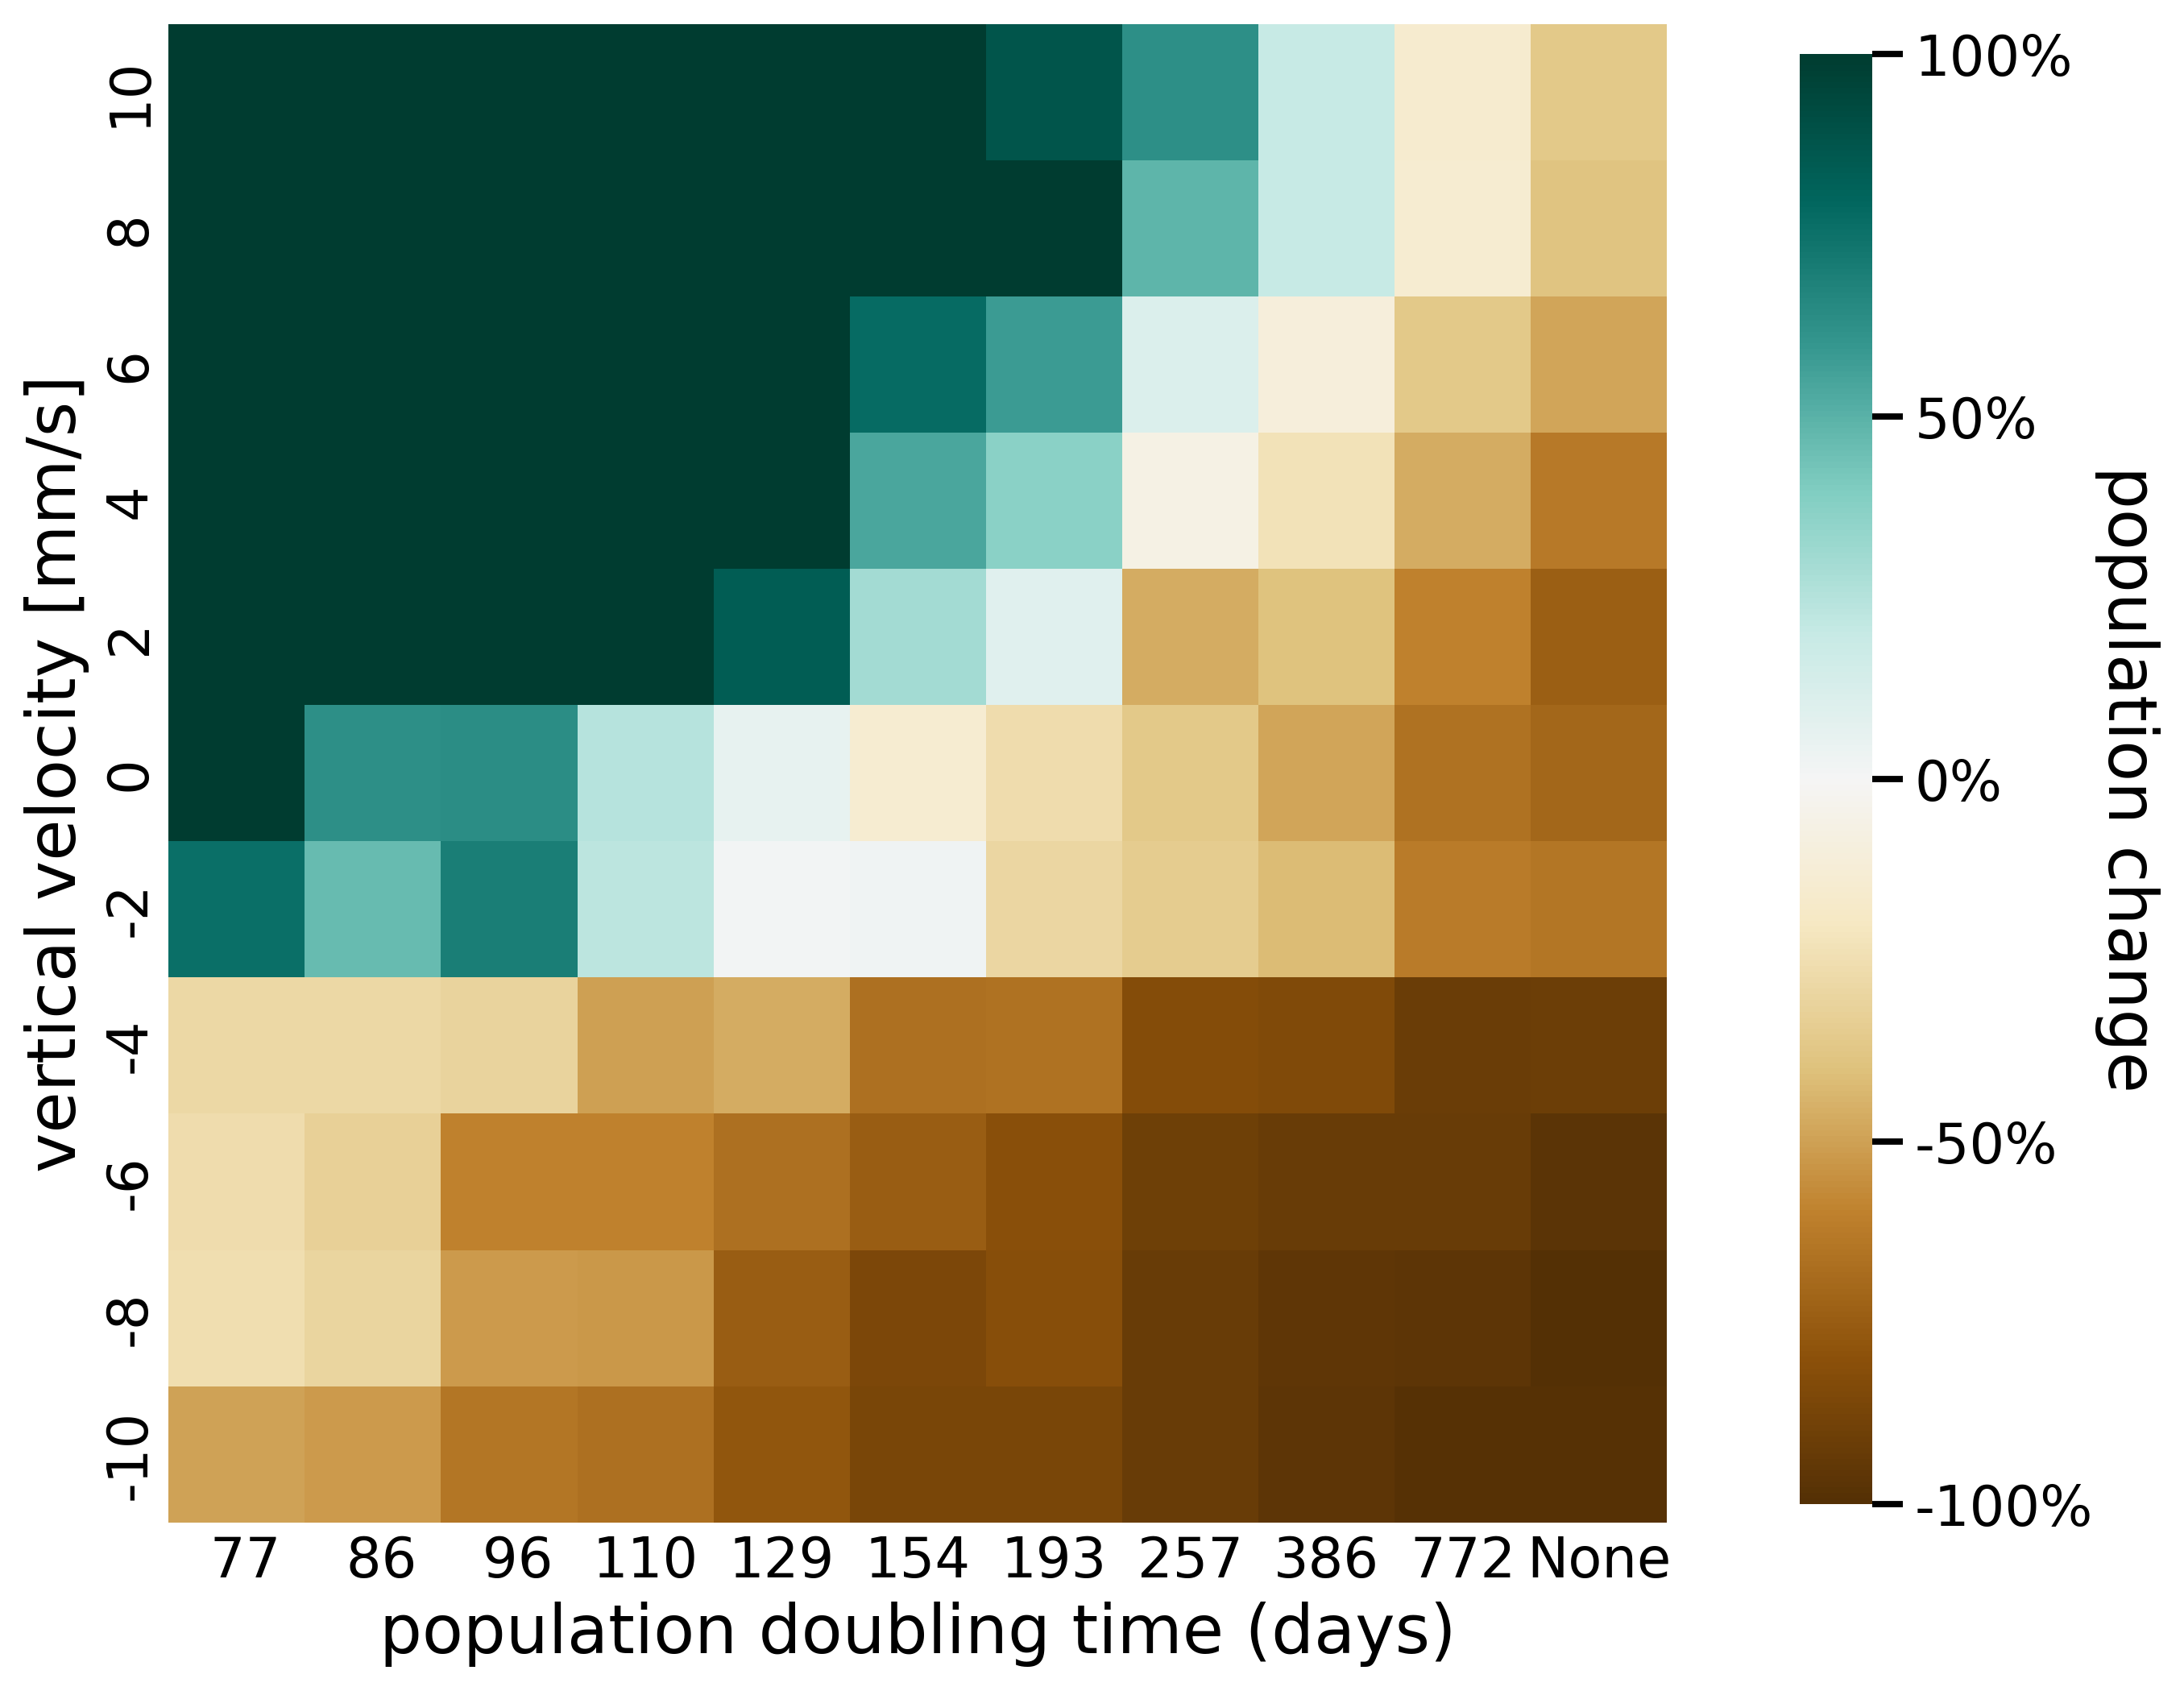
\includegraphics[width=\columnwidth]{retention_success_sa_diel.png}
    \caption[]{Relative population changes for the diel migration scenarios. Positive vertical velocities indicate an upwards drift direction. Positive population changes indicate a retention success (shown in green) while negative population changes predict a long term loss of the population (shown in brown).}
    \label{fig:diel_retention_success}
\end{figure}

The results of the retention experiments are visualized as heatmaps in fig. \ref{fig:monotonic_retention_success} and \ref{fig:diel_retention_success}.
Fig. \ref{fig:monotonic_retention_success} shows the results for the monotonic vertical migration scenarios e.g. constant sinking or rising.
Fig. \ref{fig:diel_retention_success} shows the results for the diel vertical migration scenarios. For the monotonic case a positive vertical velocity indicates an upwards motion. For the the diel case a positive vertical velocity means that the particles are moving upwards during the day and downwards during the night.
Each pixel in the heatmap represents a scenario with a specific vertical velocity and a specific reproduction rate. The coloring indicates the relative population change after one year. A positive (green) value is consider a successful retention while a negative (brown) value indicates that the population is going to die out.

The first thing that we wish to highlight is that the population successfully retains itself in certain scenarios. For the case of the monotonic migration we see a trend that the populations with higher positive velocities and higher growth rates are more successful in retaining themselves.
For the case of the diel migration we see a trend to higher vertical velocities both upwards and downwards.

Another thing that we would like to highlight is that populations with no reproduction are all unsuccessful in retaining themselves.

We would also like to note that a net-zero-growth rates represent the cases in which the growth is equal to the net losses.
Hence, the white pixels or the boundary between green and brown can be interpreted as an estimate for the total relative losses due to outwashing, dry-out when stranded, and light starvation.

\medskip

In the scenario where we disabled reproduction for stranded particles we found that the population was unable to retain itself in all tested parameterizations.





\subsubsection*{Where do they survive?}

\begin{figure}
    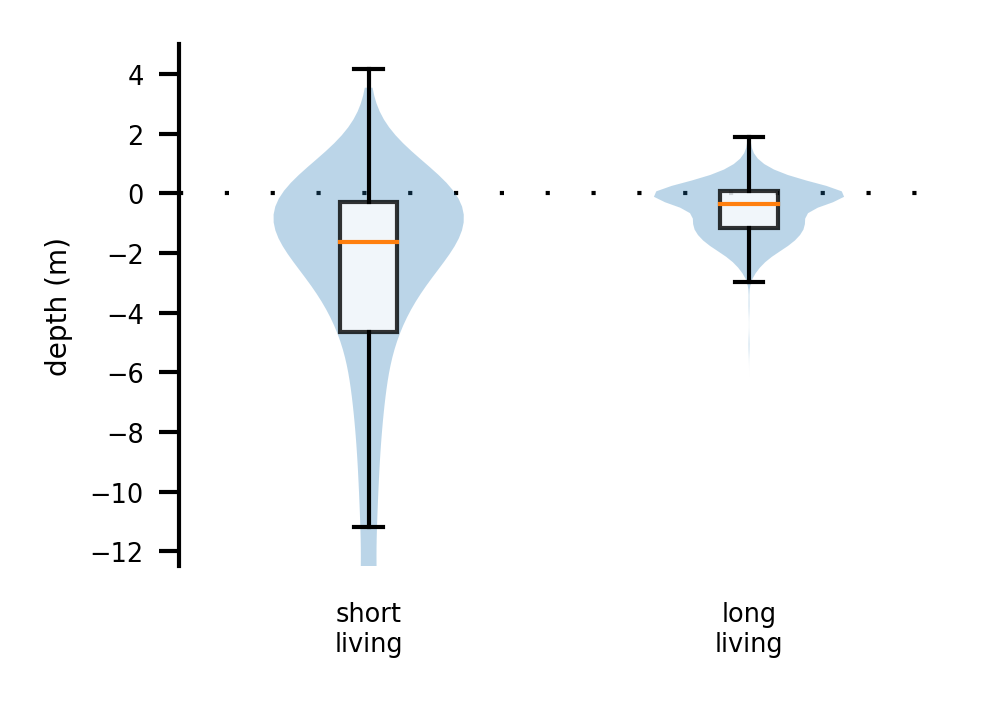
\includegraphics[width=\columnwidth]{retention_boxplot.png}
    \caption[]{Box and violing plot showing the vertical distribution of particles.  Short-living are those younger then 3 months and long-living all those older then that. Depth is measure relative to the current water surface with positive numbers being above the water surface i.e. stranded on the shore.}
    \label{fig:migration-long-vs-short}
\end{figure}

We are now taking a closer look at the subset of pytoplankton that was able to retain themselves.
In fig. \ref{fig:migration-long-vs-short} we see a box plot comparing the average water depth at particle location for the long living and short living subset. The long living being older then three months.
Depth is measured relative to the water surface. Hence, a value above zero indicate that the particle is stranded on the shore.
We can clearly see that the long living subset predominantly lives in shallower water.

\begin{figure}
    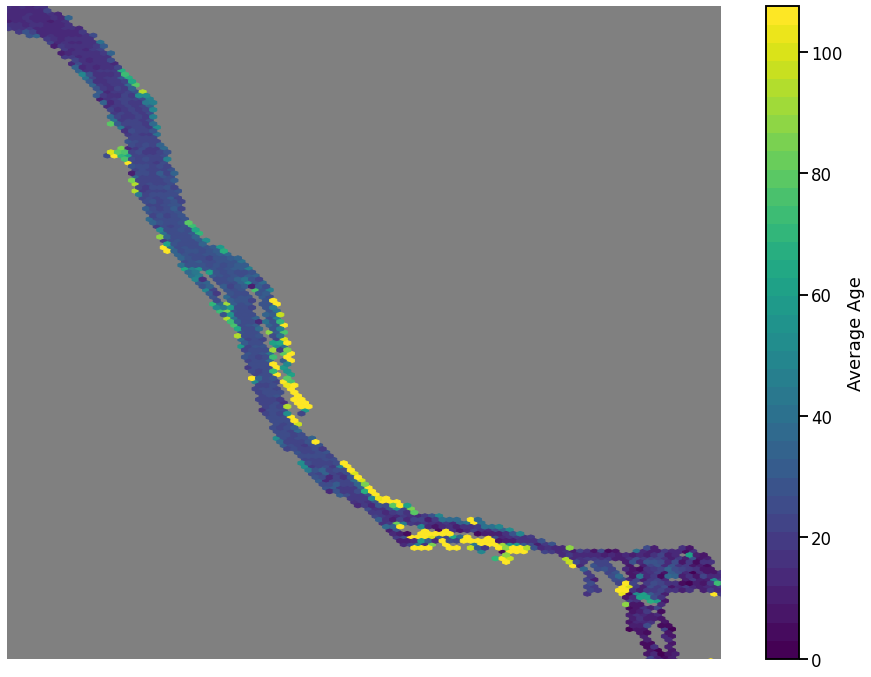
\includegraphics[width=\columnwidth]{heatmap.png}
    \caption[]{Hexbin heatmap showing average particle age per bin showing the brackish area of the Elbe downstream of the harbor.  Yellowish colors indicate an average age of over three months. \texttt{add labels and maybe use a different colormap?}}
    \label{fig:migration-long-vs-short-heatmap}
\end{figure}

This is further supported by fig. \ref{fig:migration-long-vs-short-heatmap}.
Here we see a hex-bin-plot of the estuary. The coloring shows the average age of the particles in the bin.
Bins with an average age of over three months are shown in a yellowish color.
These yellow areas can exclusively be found along the shores in shallow areas.
The major areas being Mühlenberger Loch (a), Wedeler Geest (b) and the Hasseldorfer Binnenelbe (c). We can also find minor areas at the river mouths of the Wischhafener Süderelbe (d), Ruthenstrom, and Stör (e). \texttt{labeling not yet added}
\texttt{add a show zoom in with water depth?}





% \textbf{upstream migration}

% \begin{figure}
%     \includegraphics[width=\columnwidth]{example-image-a}
%     \caption[]{particle counts in upstream statistical polygons}
%     \label{fig:upstream-migration-statistical-poly-counts}
% \end{figure}


% In the upstream migration experiment we divide the estuary in short ($\sim 50km$) sections.
% We release particles in all of these sections and count their occurrence in other sections.
% As previously described - in fig \ref{fig:upstream-migration-statistical-poly-counts} we see the 
% the particle counts for the two upstream sections from the release location.
% We consider upstream migration to happen when plankton moves two sections up and is able to retain itself there.
% \texttt{Do I need to explain why two polygons and why being there only briefly won't work?}

% \texttt{No results yet with the proper dispersion model. 
%         In the previous run upstream migration did not occur and was considered 
%         to be a negligible mechanism in the retention process.
%         However, this might chance with the enabling of tidal pumping mechanisms.}



\section*{Discussion}
%------------------------------------------------------------------------------
%------------------------------------------------------------------------------

\subsection*{Interpretation and contextualization of Results}

\subsection*{Interpretation of the results}
The range of growth rates that we found to be necessary for survival are small compared to those typically realized in nature where plankton populations can double their size in a day in ideal conditions.
Our model is simplistic in the sense that we do not include any nutrient limitation which are assumed to drastically decrease the growth rates compared to ideal conditions. 
Nevertheless, the growth rates that we found to be necessary are still much smaller compared to those typically realized in nature (cite).

The importance of shallow near-shore areas for retention has been suggested several times by our findings. 
We assume that this is for the following reasons.
Plankton that lives in this area falls dry on the shore on a regularly due to the tides basis. Hence, they are not moving downstream for a large portion of the day.
We further see that positively buoyent plankton is more successful in retaining themselves. 
This is likely due to the fact that they are more likely be washed up high up at shore where the water reaches them less frequently.
This effect is emphasized in flatter regions.
Here the distance between the wash margin and deeper waters that do not fall dry is larger. 
We assume that this effect would be further emphasized if we were to represent stokes drifts in our model even though wind forcing on the surface water is included.

Initially we expected that negatively buoyant plankton would be more successful in retaining themselves.
Sinking particles have a reduced downstream velocity as they tend to get stuck on the ground more often.
Additionally, the bottom water layer in the Elbe typically has higher upstream velocity comparts to the upper water column.
However, they still seem to be less successful than positively buoyant particles.
Examining our model we think  that this is because they tend to quickly aggregate in deep waters with little to no light where they are unable to sustain themselves and ultimately die out.
This is hinting at the negative impact of dredging on sinking plankton as it both increases the volume of deep water and increases turbidity reducing the volume of illuminated water.

We find it interesting to see that in the case of diel migration success does not seem to depend on whether they are moving up during the day or the night.
We assume that this is to a large part due to them only surviving in shallow near-shore waters where light limitation does not play a role.
We think the reason for higher success with higher vertical velocities is similar to the constant vertical velocity case.
When the upwards diel migration aligns with a high tide the particles are more likely to be stranded far out onto the shore decreasing their risk to be washed out quickly.
The higher the upwards velocities the higher the chance to be in the outmost part of the water body during high tide
However, we also want to note that our light limitation model is very simplistic to keep the model complexity low.
For plankton to be not light limited they only need to be above a depth of one meter in the high turbidity water of the Elbe unregarded of current illumination conditions and local turbidity.
We therefore think that a more realistic light limitation model might introduce a positive bias towards those particles that move upwards during the day.

\subsection*{Limitations of the model}

One major limitation of our model is the lack of nutrient limitation or the lack of a realistic ecosystem model in general.
This could have been done by coupling our Lagrangian model online to an Eularian model that would have advected changes in concentrations fields by biotic activity throughout the model domain.
However, this would have drastically increased both developing and computational time to a point where it would have been infeasible in our time frame and due to the lack of appropriate validation data.
The key draw back of this is that growth rates could only be modeled as a constant rate assuming an "ad libitum" environment at all times.
This introduces systematic errors in the population growth as areas which are beneficial for retention might in reality quickly run out of nutrients and could not sustain the growth conditions necessary to sustain the local population.

Another major limitation is the lack of any sub-grid-resolution structure on the shores - especially vegetation.
In our representation we assume perfectly flat surfaces with an median distance between nodes of approximately 60m.
This "polished" model representation is assumed to cause a strong negative bias towards retention success as some plankton could easily stick to the vegetation or other cavities caused by the sub-grid-resolution structure and reseed the area.

While our model does have a sedimentation and resuspension mechanic based on critical sheer velocities we still assume a static bathymetrie with sediments not able to move or bury particles. 
This maskes potential losses due to particles being buried but also decreases resuspension times.

\subsection*{Outlook}

Our results clearly suggested the importance of shallow near-shore areas for the survival of phytoplankton in the Elbe estuary.
After our initial experiments suggested this, we considered improving our model to resolve additional ecosystem interactions especially nutrient limitation.
This would allow us to predict the population dynamics more realistically to the point where we would be able to quantize importance of shallow areas more accurately.
However, the main limitation to do so was the lack of validation data for these regions. 
Almost all chlorophyll data is gather in the center of the river.
While we consider the general trend shown by our model to be true - shallow areas are essential for survival. We can not quantify the effect of changes in these areas that might be caused by future dredging, diking or restoration attempt.
To do this, we first require more specially resolved data for these areas.

We were also surprised by our finding that sinking particles have a harder timer surviving in the estuary. 
Since several decades the yearly average chlorophyll concentration in the Elbe estuary concentrations declined (cite) while upstream concentrations do not show this effect.
The reasons for this are not yet fully understood but one potential reason is the increase in dreading activities.
These increases the average turbidity reducing the water volume where phytoplankton is able to grow.
A large fraction of the upstream phytoplankton consists of diatoms (cite).
Diatoms typically have negative buoyancies (cite) making them especially vulnerable to sinking to light limited waters.

Another mechanism that might in part explain this effect is but is not yet explored in our model is the phytoplankton stickiness (cite). 
Phytoplankton especially blooming one has been shown to be sticky due to exudates (cite Alenka Male 1993).
In combination with increased turbidity this losses due to plankton aggregates sticking to negatively buoyant suspended matter and subsequently sinking to the ground where they are starved of light.
We are curious to which extend these mechanisms might explain the phytoplankton losses in the dreadged areas of the estuary and suggest both a field and modling study. A field study could provide estimates on suspended matter concentration dependant aggregation speeds of phytoplankton and their sinking velocities. While the model study might create estimates on chlorophyll concentration losses caused by this effect.


\section*{Conclusion}

We saw that reproducing phytoplankton is able to maintain their population strain without up- or downstream reseeding under certain conditions.
We were also able to give a first estimate on the growth rates necessary for survival of the population depending on their buoyancy and their respective outwashing losses.
We also saw that the population is ultimately washed out and perishes if we suppress reproduction.
The same is true if we do not suppress reproduction completely but only for particles currently not floating in the water body indicating the importance of the shores for retention.
To investigate this further we looked at the average water depth of long living particles and the areas where they are found which further indicated the importance of shallow areas for retention.

We suggest further sampling to measure chlorophyll concentrations in shallow waters - specifically at Mühlenberger Loch and Hasseldorfer Binnenelbe - to quantify the importance of these areas on the general population health.
                


